\documentclass[aspectratio=169]{beamer}

\mode<presentation>
{
  \usetheme{default}
  \usecolortheme{default}
  \usefonttheme{default}
  \setbeamertemplate{navigation symbols}{}
  \setbeamertemplate{caption}[numbered]
  \setbeamertemplate{footline}[frame number]  % or "page number"
  \setbeamercolor{frametitle}{fg=white}
  \setbeamercolor{footline}{fg=black}
} 

\usepackage[english]{babel}
\usepackage[utf8x]{inputenc}
\usepackage{tikz}
\usepackage{courier}
\usepackage{array}
\usepackage{bold-extra}
\usepackage{minted}
\usepackage[thicklines]{cancel}

\xdefinecolor{dianablue}{rgb}{0.18,0.24,0.31}
\xdefinecolor{darkblue}{rgb}{0.1,0.1,0.7}
\xdefinecolor{darkgreen}{rgb}{0,0.5,0}
\xdefinecolor{darkgrey}{rgb}{0.35,0.35,0.35}
\xdefinecolor{darkorange}{rgb}{0.8,0.5,0}
\xdefinecolor{darkred}{rgb}{0.7,0,0}
\definecolor{darkgreen}{rgb}{0,0.6,0}
\definecolor{mauve}{rgb}{0.58,0,0.82}

\title[2017-11-16-dataorg-columnar]{Managing data with columnar granularity}
\author{Jim Pivarski}
\institute{Princeton University -- DIANA-HEP}
\date{November 16, 2017}

\begin{document}

\logo{\pgfputat{\pgfxy(0.11, 7.4)}{\pgfbox[right,base]{\tikz{\filldraw[fill=dianablue, draw=none] (0 cm, 0 cm) rectangle (50 cm, 1 cm);}\mbox{\hspace{-8 cm}
\includegraphics[height=1 cm]{princeton-logo-long.png}
\includegraphics[height=1 cm]{diana-hep-logo-long.png}}}}}

\begin{frame}
  \titlepage
\end{frame}

\logo{\pgfputat{\pgfxy(0.11, 7.4)}{\pgfbox[right,base]{\tikz{\filldraw[fill=dianablue, draw=none] (0 cm, 0 cm) rectangle (50 cm, 1 cm);}\mbox{\hspace{-8 cm}
\includegraphics[height=1 cm]{princeton-logo.png}
\includegraphics[height=1 cm]{diana-hep-logo.png}}}}}

% Uncomment these lines for an automatically generated outline.
%\begin{frame}{Outline}
%  \tableofcontents
%\end{frame}

% START START START START START START START START START START START START START

\begin{frame}{Nature of this talk}
\vspace{0.5 cm}
\begin{columns}
\column{1.05\linewidth}
\Large This talk isn't about how we manage data in HEP, but how we {\it might.}
\end{columns}

\vspace{0.5 cm}
\begin{itemize}\setlength{\itemsep}{0.25 cm}
\item \Large Therefore, it isn't a ``how-to'' talk but a ``what-if'' talk.
\item \Large If you have experience in this, we want to hear from you!
\end{itemize}
\end{frame}

\begin{frame}{Columnar data}
\vspace{0.25 cm}
\begin{columns}
\column{0.45\linewidth}
Serializing data in columns is an old idea in HEP:

\vspace{0.25 cm}
\begin{itemize}
\item \textcolor{darkblue}{1989:} Column-Wise-N-tuples (CWN) in PAW
\item \textcolor{darkblue}{1996:} ``split'' (columnar) C++ objects in ROOT

\vspace{0.25 cm}
\ldots

\vspace{0.25 cm}
\item \textcolor{darkblue}{2002:} MonetDB
\item \textcolor{darkblue}{2005:} C-Store (Vertica)
\item \textcolor{darkblue}{2010:} Google Dremel paper
\item \textcolor{darkblue}{2013:} Apache Parquet
\end{itemize}

\column{0.55\linewidth}
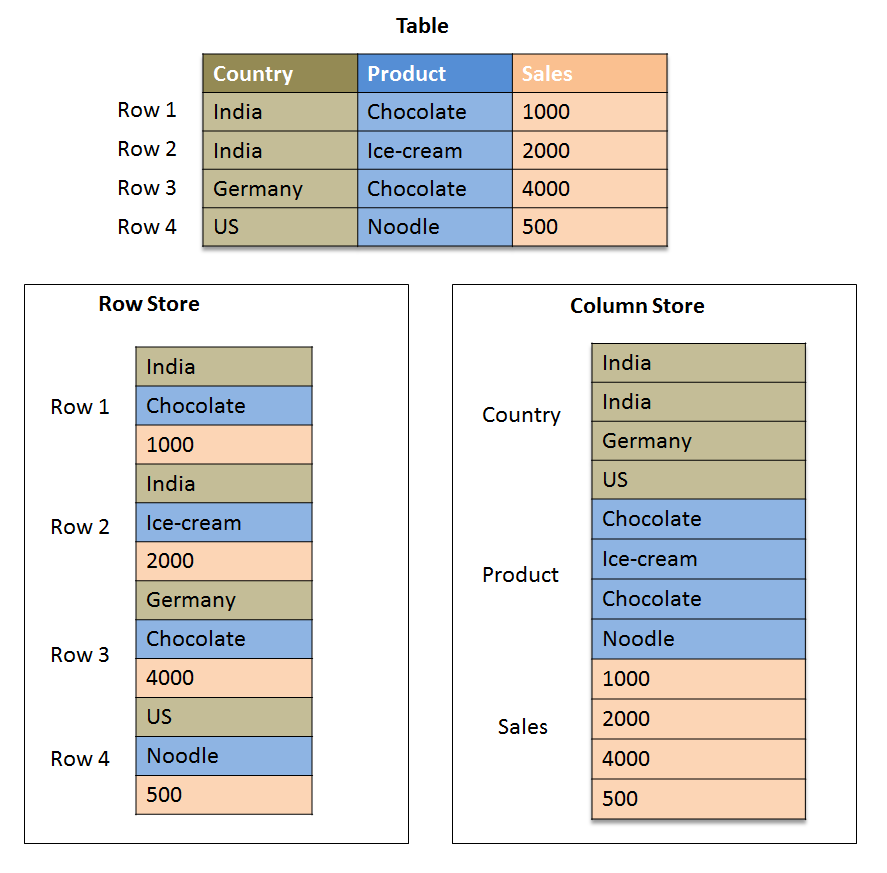
\includegraphics[width=\linewidth]{columnar-vs-rowwise-sap.png}
\end{columns}
\end{frame}







\end{document}
